\documentclass{article}
\usepackage{amsmath}
\usepackage{graphicx}
\author{Kevin Lu, Travis You}
\title{Simulation and Inference for the Generalized Toilet Paper Problem}
\begin{document}
\maketitle
\section{Introduction}
In 1984, Knuth formulated a theoretical consideration for a ``toilet paper problem" \cite{Knuth1984}, which is a generalized matchbox problem from \cite{Feller}. 

Consider two types of people using toilet paper: big-choosers and little-choosers, and a 2-roll toilet paper set. Big-choosers only uses toilet paper on the roll with more toilet paper and little-choosers only use toilet paper on the roll with less toilet paper. If both rolls have exactly the same amount of toilet paper, both types of people will randomly select a roll to use. Assume that all persons take 1 unit of toilet paper each time they use the restroom and that both rolls initially have $n$ units of toilet paper. If the amount of paper on the other roll when one roll is emptied is large, then the janitor would have plenty of time for replacement, but if that is not the case, people may run into problems.

Assume people enter the toilet independently at random, with proportion $p$ being big-choosers and proportion $q=1-p$ being little-choosers. Let $X$ be the random variable recording the number of paper left on one roll when the other roll first empties, Knuth showed that the expected value $E(X)$, denoted as $M_n(p)$, follows
\begin{equation}
    M_n(p) = n-\sum_{k=1}^{n-1} (n-k)c_k p^k q^{k-1}, 
\end{equation}
where $c_n = \binom{2n-2}{n-1}\frac{1}{n}$ is the catalan number. He has also given approximation of $M_n(p)$ for large $n$ as 
\begin{equation}
    M_n(p)=
    \begin{cases}
        \frac{q-p}{q}n+\frac{p}{q-p}+O(r^n) & \text{if }  p<1/2 \\
        \frac{p}{p-q} + O(r^n) & \text{if } p>1/2
    \end{cases}
    ,
    \label{limiting Mnp}
\end{equation}
where $r$ is any value greater than $4pq,$ which is smaller than $1$ for any $p \neq \frac{1}{2}$. The approximation in Eq.\eqref{limiting Mnp} works well when $|p-\frac{1}{2}|$ is at least of order $1/\sqrt{n}$. In that case, as $n$ is big, $O(r^n)$ is essentially 0. 

When $p$ is sufficiently close to $\frac{1}{2}$, the approximation in Eq.\eqref{limiting Mnp} does not work and $M_n(p)$ is better approximated by 
\begin{equation}
    M_n(p)=
    2\sqrt{\frac{n}{\pi}} - \frac{1}{4} \sqrt{\frac{1}{\pi n}} + O(n^{-3/2})
\end{equation}

Therefore, when little-choosers predominate, $M_n(p)$ is of order $n$; when big-choosers predominate, $M_n(p)$ is of order $1$; when little-choosers and large-choosers are of similar number, $M_n(p)$ is of order $\sqrt{n}$. Moreover, there is a significant drop near $p=\frac{1}{2}$ for large $n$. 

In this paper, we're going to investigate further about the distribution of leftover amount $X$. Moreover, we're going to generalize the problem into a problem involving 3 and more rolls of toilet paper to test the claim that ``to solve the shortage of toilet paper when all other rolls empties, we just need to pile more rolls of toilet papers in the restroom.''
\section{2-Roll Simulation}
\begin{figure}[ht]
    \centering
    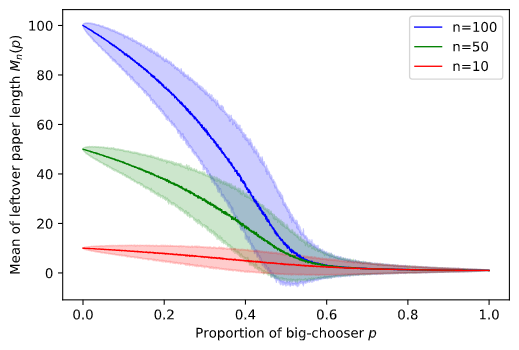
\includegraphics[width=8cm]{Mnp-2roll.png}
\end{figure}
\bibliographystyle{unsrt}
\bibliography{MyCollection.bib}
\end{document}